\documentclass[10pt,a4paper]{article}
% Meshtastic Gateway user guide. Built with:  pdflatex user_guide.tex  (twice; three times for the contents)
% The screenshots are in guide_img/ and are made with guide_shots.py from an invented demo database.
\usepackage[T1]{fontenc}
\usepackage[utf8]{inputenc}
\usepackage{mathptmx}
\usepackage[scaled=.92]{helvet}
\usepackage{courier}
\usepackage{microtype}
\usepackage[a4paper,margin=2.0cm,top=2.3cm,bottom=2.2cm,headsep=0.5cm]{geometry}
\usepackage{graphicx}
\usepackage{xcolor}
\usepackage{booktabs}
\usepackage{tabularx}
\usepackage{array}
\usepackage{enumitem}
\usepackage{caption}
\usepackage{float}
\usepackage{fancyhdr}
\usepackage{textcomp}
\usepackage{amsmath}
\usepackage{amssymb}
\usepackage{tikz}
\usetikzlibrary{arrows.meta,positioning}
\usepackage{tocloft}
\setlength{\cftbeforesecskip}{0.6pt}
\renewcommand{\cftsecfont}{\normalfont}
\renewcommand{\cftsecpagefont}{\normalfont}
\usepackage[hidelinks]{hyperref}

\definecolor{accent}{HTML}{0369A1}
\definecolor{boxbg}{HTML}{F1F6FA}
\definecolor{warnbg}{HTML}{FFF7E8}
\definecolor{warn}{HTML}{B45309}
\definecolor{ackY}{HTML}{198754}
\definecolor{ackS}{HTML}{B7791F}
\captionsetup{font=small,labelfont=bf,labelsep=period,justification=justified,singlelinecheck=false}
\setlist{itemsep=1.5pt,topsep=3pt,parsep=0pt}
\setlength{\parindent}{0pt}
\setlength{\parskip}{4.5pt plus 1pt}
\renewcommand{\arraystretch}{1.15}
\setcounter{tocdepth}{1}
\pagestyle{fancy}
\fancyhf{}
\fancyhead[L]{\small\itshape Meshtastic Gateway --- how to read and use the web page}
\fancyhead[R]{\small\itshape User guide, version 1.8 --- November 2026}
\fancyfoot[C]{\small\thepage}
\renewcommand{\headrulewidth}{0.3pt}
\hypersetup{pdftitle={Meshtastic Gateway - User guide},pdfauthor={Otso Laakso, OH2GAX}}

\newcommand{\km}{\,km}
\newcommand{\dB}{\,dB}
\newcommand{\MHz}{\,MHz}
\newcommand{\ui}[1]{\textsf{\small #1}}            % a word on the screen: button, switch, card title
\newcommand{\lead}[1]{\textbf{#1}\enspace}           % run-in paragraph head
\newcommand{\cmd}[1]{\texttt{#1}}
\newcommand{\fig}[3]{\begin{figure}[H]\centering\includegraphics[width=#2\textwidth]{guide_img/#1}\caption{#3}\end{figure}}
\newcommand{\figpair}[5]{\begin{figure}[H]\centering
  \begin{minipage}[t]{0.485\textwidth}\centering\includegraphics[width=\textwidth]{guide_img/#1}\end{minipage}\hfill
  \begin{minipage}[t]{0.485\textwidth}\centering\includegraphics[width=\textwidth]{guide_img/#2}\end{minipage}
  \caption{#5}\label{#3}\end{figure}}
\newcommand{\infobox}[2]{\par\smallskip\noindent\fcolorbox{accent!60}{boxbg}{\begin{minipage}{\dimexpr\textwidth-2\fboxsep-2\fboxrule\relax}\small
  \textbf{#1}\enspace #2\end{minipage}}\par\smallskip}
\newcommand{\warnbox}[2]{\par\smallskip\noindent\fcolorbox{warn!60}{warnbg}{\begin{minipage}{\dimexpr\textwidth-2\fboxsep-2\fboxrule\relax}\small
  \textbf{#1}\enspace #2\end{minipage}}\par\smallskip}
\newcommand{\ackY}{\textcolor{ackY}{\textbf{Y}}}
\newcommand{\ackS}{\textcolor{ackS}{\textbf{S}}}

\begin{document}
\thispagestyle{plain}
\begin{center}
{\small Meshtastic Gateway project \quad$\cdot$\quad User guide, version 1.8 \quad$\cdot$\quad 16 November 2026}\par\vspace{10pt}
{\LARGE\bfseries Meshtastic Gateway}\par\vspace{5pt}
{\large\bfseries How to read and use the web page:\\ nodes, messages, the map, services and the gateway itself}\par\vspace{8pt}
{\normalsize Otso Laakso (OH2GAX)}\par
{\small Heltec V3 / V4 over WiFi \quad$\cdot$\quad Raspberry Pi \quad$\cdot$\quad \url{https://github.com/oh2gax/meshtastic_gateway}}
\end{center}
\vspace{2pt}

\infobox{In short.}{A Meshtastic radio (a Heltec V3 or V4) sits on the home WiFi. The gateway, a small Python program on a Raspberry Pi, keeps a connection to it open day and night, stores everything the radio hears in a database and shows it in a web page that any computer or phone on the home network can open. In one page you can:
\begin{itemize}[leftmargin=1.2em]
\item \textbf{see who is on the mesh} --- every node heard, how strong and how many hops away it is, where it is on a map, and the exact path to it with a traceroute (Sections~\ref{sec:nodes}, \ref{sec:map} and~\ref{sec:trace});
\item \textbf{read and send messages} --- private direct messages with delivery marks, a chat view per node, and the public channels (Sections~\ref{sec:inbox}--\ref{sec:send});
\item \textbf{answer questions from the field automatically} --- a node can send \cmd{wx EFHK}, \cmd{taf EFHK}, \cmd{cmd solar}, \cmd{cmd wspr} or \cmd{cmd trace} to the gateway and gets the weather, the solar conditions, the WSPR propagation or the route to itself back over the mesh (Section~\ref{sec:services});
\item \textbf{keep the gateway healthy} --- connection status, clean-up of nameless nodes and a raw packet view (Sections~\ref{sec:status}--\ref{sec:debug}).
\end{itemize}
Section~\ref{sec:mesh} explains Meshtastic as far as needed to read the page; Section~\ref{sec:pi} is for the person who runs the gateway, Section~\ref{sec:limits} lists what the page cannot tell and Section~\ref{sec:quick} is a one-page quick reference.}

\infobox{About the figures.}{All figures are screenshots of the real page, but filled with an \emph{invented demo database}: the nodes (\emph{Harbour Relay}, \emph{Hill Top Router} \dots), their positions and the messages are made up, so that nobody's private messages or home location appear in this guide. In the map figure the background is a plain outline of the coast; on the real page it is a detailed street map. The times in the figures are UTC; the page can also show local time (Section~\ref{sec:page}).}

{\small\tableofcontents}

\newpage
\section{Meshtastic in a nutshell}\label{sec:mesh}

\subsection{Nodes, the mesh and hops}
\lead{Meshtastic} is an open-source project that turns small, cheap LoRa radios into a text-messaging network that needs no mobile network, no internet and no licence. In Europe it uses the 868\MHz band. A radio running Meshtastic is a \emph{node}. Nodes can be handheld, on a roof, in a car or solar-powered on a hill.

\lead{The mesh.} When a node sends a packet, every node that hears it can send it on again. That is how a message gets further than one radio could carry it. Each packet carries a \emph{hop limit} (normally 3, at most 7): every relay lowers it by one, and at zero the packet is not sent on any more. A node also remembers what it has already relayed, so a packet does not circle round the mesh.

\lead{Hops.} The packet also says what its hop limit was when it was sent (\emph{hop start}). The difference is the number of hops it travelled before it reached the gateway: \textbf{0~hops} means the gateway heard the sender directly, 2~hops means two other nodes relayed it on the way. Older firmware does not send the hop start; then the page shows ``---''.

\lead{Who is who.} Every node has a fixed \emph{node ID} such as \cmd{!5e10a001} (eight hexadecimal digits, from the radio's hardware) and a \emph{long name} and \emph{short name} that its owner chooses, for example \emph{Harbour Relay} and \emph{HRB1}. The names travel in separate \emph{NodeInfo} packets that are sent now and then; until one of them has been heard, a node is known only by its ID.

\subsection{Channels, broadcasts and direct messages}
\lead{Channels.} A radio has up to eight channel slots (index 0--7). Slot~0 is the \emph{primary} channel; the default public channel of Meshtastic is a primary channel with a well-known key, so everybody can read it. Further \emph{secondary} channels (for example a club channel) have their own name and key: only nodes with the same key can read them.

\lead{Broadcast.} A message sent to everybody on a channel. Every node with that channel shows it. Broadcasts are not acknowledged.

\lead{Direct message (DM).} A private message to one node. With current firmware (2.5 and later) it is encrypted with the receiver's public key (PKI), so the relays cannot read it, whatever channel they use.

\lead{Acknowledgement (ACK).} The sender of a DM asks for an acknowledgement. When the destination receives the message, it sends a small \emph{routing} packet back: that is the end-to-end ACK. There is a second, weaker kind: when the sending radio hears one of its neighbours \emph{relay} its message, it takes that as an \emph{implicit ACK} --- the message has left the radio and is on its way, but nobody knows yet whether the destination got it. The gateway keeps the two apart (Section~\ref{sec:outbox}).

\subsection{How the gateway works}
\begin{figure}[H]\centering
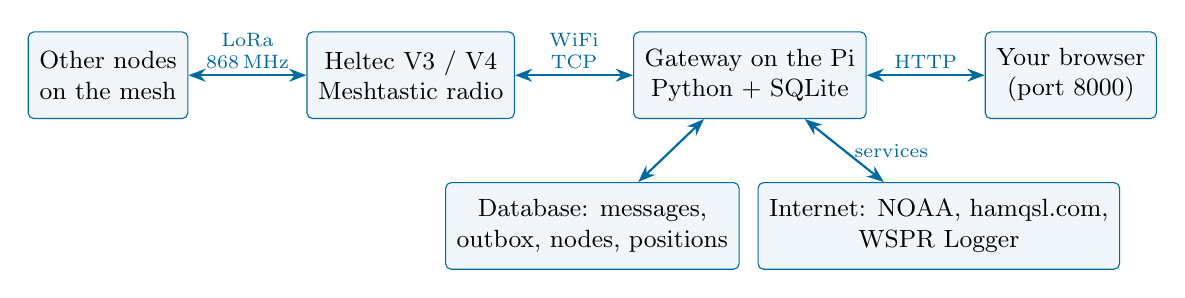
\begin{tikzpicture}[node distance=8mm and 15mm, every node/.style={font=\small}, box/.style={draw=accent, fill=boxbg, rounded corners=2pt, align=center, inner sep=4pt, minimum height=11mm},
  arr/.style={{Stealth[length=2.2mm]}-{Stealth[length=2.2mm]}, accent, thick}, lbl/.style={above, align=center, font=\scriptsize, inner sep=2pt}]
\node[box] (mesh) {Other nodes\\on the mesh};
\node[box, right=of mesh] (radio) {Heltec V3 / V4\\Meshtastic radio};
\node[box, right=of radio] (gw) {Gateway on the Pi\\Python + SQLite};
\node[box, right=of gw] (br) {Your browser\\(port 8000)};
\node[box, below=of gw, xshift=-20mm] (db) {Database: messages,\\outbox, nodes, positions};
\node[box, below=of gw, xshift=24mm] (net) {Internet: NOAA, hamqsl.com,\\WSPR Logger};
\draw[arr] (mesh) -- node[lbl]{LoRa\\868\,MHz} (radio);
\draw[arr] (radio) -- node[lbl]{WiFi\\TCP} (gw);
\draw[arr] (gw) -- node[lbl]{HTTP} (br);
\draw[arr] (gw) -- (db); \draw[arr] (gw) -- node[right,font=\scriptsize]{services} (net);
\end{tikzpicture}
\caption{From the mesh to the page. The gateway talks to the radio over the home WiFi; the radio does all the radio work.}
\end{figure}

\lead{Always listening.} The gateway keeps a TCP connection to the radio's WiFi interface open. Every packet the radio receives is passed to the gateway, which
\begin{itemize}[leftmargin=1.2em]
\item stores \textbf{text messages}: direct messages for the Inbox and Chat, broadcasts for the Broadcast page;
\item updates the \textbf{node list}: when each node was last heard, its signal strength, hops and position, and its names and hardware model from the radio's own node database (refreshed every 30 seconds);
\item stores \textbf{positions}, so the map can draw tracks;
\item matches \textbf{routing packets} to the messages it sent, to mark them delivered;
\item keeps the last 300 packets in raw form for the Debug page.
\end{itemize}

\lead{Sending.} Messages you write are first put in a queue, the \emph{outbox}. The gateway hands them to the radio one at a time, about one per second, and then follows the ACK. If the radio cannot be reached, the gateway reconnects by itself every few seconds.

\lead{Services.} When a node sends a service command as a direct message, the gateway fetches the answer from the internet and sends it back as a DM. This happens in the background, so the radio keeps receiving while the answer is fetched.

\infobox{Words used in this guide.}{\textbf{Node}: a Meshtastic radio. \textbf{Node ID}: its fixed address, \cmd{!} and eight hex digits. \textbf{DM}: direct (private) message. \textbf{Broadcast}: a message to everybody on a channel. \textbf{Hops}: how many relays a packet passed on its way to the gateway (0 = heard directly). \textbf{RSSI}: received signal strength in dBm (about $-40$ is very strong, $-120$ is at the limit). \textbf{SNR}: signal-to-noise ratio in dB; LoRa can still decode below 0\,dB, down to about $-20$\,dB. \textbf{ACK}: acknowledgement of a DM. \textbf{UTC}: the page shows times in UTC unless you switch to local time.}

\section{The page at a glance}\label{sec:page}
\fig{navbar.jpg}{1.0}{The top bar. From the left: the pages, the unread-messages badge, What's new, the UTC / local time switch, the theme menu and Send.}

\lead{The top bar} stays at the top of every page:
\begin{itemize}[leftmargin=1.2em]
\item the \textbf{title} (it opens Active Nodes) and the pages: \ui{Inbox}, \ui{Outbox}, \ui{Active Nodes}, \ui{Broadcast}, \ui{Chat}, \ui{Map}, \ui{Debug}, \ui{Status} and \ui{Services}. The page you are on is highlighted;
\item \ui{Broadcast} turns \textbf{red with a red dot} when a new broadcast has arrived since you last opened the Broadcast page;
\item the red \textbf{envelope badge} (``2 new'') appears when there are unread direct messages; it opens the Inbox. It is checked every 5 seconds, so it appears without reloading the page;
\item the \textbf{sparkle button} opens \ui{What's new}; a red dot on it means notes you have not read yet (Section~\ref{sec:whatsnew});
\item the \textbf{clock} button (\ui{UTC} / \ui{Local}) chooses the time zone of all times, see below;
\item the \textbf{theme} button (a half-filled circle, sun or moon) opens the menu \ui{Auto} / \ui{Light} / \ui{Dark} (Section~\ref{sec:theme});
\item \ui{Send} opens the form for a new message (Section~\ref{sec:send}).
\end{itemize}
On a narrow screen the page names fold into the \ui{$\equiv$} menu button (Figure~\ref{fig:phone}).

\lead{The footer} shows the IP address of the radio, the version of the gateway (click it for What's new) and whether the times are in UTC or local time.

\lead{UTC or local time.} The \ui{UTC} button in the top bar (on a phone: \ui{Time} in the \ui{$\equiv$} menu) switches every time on every page between UTC and the local time of the computer or phone you are using, for example Finnish time (UTC\,+\,2, in summer UTC\,+\,3). The button shows the zone in use; pointing at any time shows it in the other zone. The choice is remembered in the browser. The gateway itself always stores UTC, and service replies such as METAR and WSPR keep their own UTC (\cmd{Z}) times.

\lead{Auto-refresh.} Most pages have a small \ui{Off / 10s / 30s / 60s} selector with a circular-arrow icon. It reloads the page at that interval. The choice is remembered per page; the Outbox starts at 10\,s, the others at Off. While you are typing a message the reload waits, so nothing you write is lost.

\figpair{phone_outbox.jpg}{phone_menu.jpg}{fig:phone}{}{On a phone. Left: the Outbox. Right: the menu opened with the \ui{$\equiv$} button.}

\section{Active Nodes}\label{sec:nodes}
\fig{nodes.jpg}{1.0}{Active Nodes with the window \ui{1d}: twelve nodes heard in the last day, sorted by distance from the gateway (the blue $\blacktriangle$ in the \ui{Distance} heading).}

The start page lists every node heard within the chosen \textbf{window}: \ui{2h} (the default), \ui{6h}, \ui{1d}, \ui{1w} or \ui{1m} (30 days). The chips next to the title repeat the window and the number of nodes (\ui{count=12}).

\begin{tabularx}{\textwidth}{@{}lX@{}}
\toprule
Column & Meaning \\
\midrule
Last seen & When any packet from the node was last received (UTC or local time, see Section~\ref{sec:page}). \\
Node & The node ID. \\
Name & Long name and, in brackets, the short name. A node whose names have not been heard yet is shown by its ID (\cmd{!5e10a009} in the figure). \\
HW & The hardware model the node reports, e.g.\ \cmd{HELTEC\_V3}, \cmd{RAK4631}, \cmd{TRACKER\_T1000\_E}. \\
RSSI, SNR & Signal strength and signal-to-noise ratio of the last packet received from it. For a node more than 0~hops away these describe the \emph{last relay}, not the node itself. \\
Pos & \textcolor{ackY}{Y} when the node has sent a position, --- when not. \\
Hops & Hops of the most recent packet: 0 = heard directly, --- = unknown. \\
Distance & How far the node's last position is from the gateway's own position, in km; --- when either position is unknown. \\
\bottomrule
\end{tabularx}

\lead{Sorting.} Click a column heading --- \ui{Last seen}, \ui{Name}, \ui{RSSI}, \ui{SNR}, \ui{Hops} or \ui{Distance} --- to sort the list by it; click again to reverse the order. The heading shows $\blacktriangle$ or $\blacktriangledown$. Nodes without a value (no position, no name \dots) always come last. The page remembers the order, also when it refreshes itself; at first it is the newest first.

The buttons at the end of a row are, from the left: the green \textbf{traceroute} button with its small \ui{$\blacktriangledown$} (Section~\ref{sec:trace}), the \textbf{map} button, which opens the Map zoomed to the node with its details open (grey when the node's position is not known), \ui{Chat} with that node and the \ui{Send} form addressed to it.

\infobox{Reading the list.}{Nodes with 0~hops and a good SNR are your direct neighbours: these are the ones that carry your messages into the mesh. A node that is heard only with 3--4~hops is far away or behind hills; DMs to it take longer and are more often marked \ackS{} (Section~\ref{sec:outbox}).}

\section{Inbox}\label{sec:inbox}
\fig{inbox.jpg}{1.0}{The Inbox. The two newest messages are unread: bold, with a yellow background and a red dot.}

The Inbox shows the \textbf{direct messages} sent to the gateway, newest first. Each row has the time, the sender (name, ID and hops of that message), the text and the RSSI and SNR at which it was received.

\begin{itemize}[leftmargin=1.2em]
\item \textbf{Unread} messages are bold with a yellow background and a red dot. They also light the envelope badge in the top bar.
\item The green tick \ui{Mark read} marks one message read; \ui{Mark all read} marks them all. Opening the \ui{Chat} with a node marks its messages read too.
\item \ui{Chat} opens the conversation with the sender, \ui{Reply} the Send form with the sender already chosen.
\item The red bin deletes the message from the gateway's database (not from any radio). You are asked to confirm.
\item \ui{50 / 200 / 1000} sets how many messages are listed.
\end{itemize}
Service commands (\cmd{wx EFHK} and the others, Section~\ref{sec:services}) are not shown in the Inbox: they are commands to the gateway, not messages to you.

\section{Outbox and the delivery marks}\label{sec:outbox}
\fig{outbox.jpg}{1.0}{The Outbox: \ackY{} delivered (with the hops the acknowledgement travelled back), \ackS{} sent without confirmation and \dots\ still waiting.}

The Outbox lists the direct messages the gateway has sent or is about to send, newest first, with the destination, the text and the \textbf{Ack} mark. (Broadcasts are on the Broadcast page.) It refreshes itself every 10 seconds by default, so you can watch a mark change.

\begin{center}
\begin{tabularx}{\textwidth}{@{}>{\centering\arraybackslash}p{1.1cm}X@{}}
\toprule
Ack & Meaning \\
\midrule
\ackY & \textbf{Delivered.} The destination node itself acknowledged the message (end-to-end ACK). Next to it: how many hops the acknowledgement travelled back, e.g.\ \ui{Y 1 hop}; pointing at it shows the RSSI and SNR of its last hop. \\
\ackS & \textbf{Sent, not confirmed.} The radio sent the message, but no ACK came from the destination. This covers three cases: an \emph{implicit} ACK (a relay was heard passing the message on), \emph{no ACK} at all after the radio's retries or within 3 minutes, and a \emph{negative} ACK (for example no route, or the destination's key unknown). \\
\dots & \textbf{Waiting.} Sent within the last 3 minutes and no outcome yet. \\
--- & \textbf{Not applicable.} The radio never accepted the message, so there is nothing to acknowledge; the reason is shown in red under the row. \\
\bottomrule
\end{tabularx}
\end{center}

\warnbox{\ackS{} does not mean lost.}{The destination may well have received the message and its ACK was lost on the way back, or the message reached a relay and then the destination later. In the figure the DM to \emph{City Roof} was passed on by a relay (implicit ACK) and the one to \emph{Island Solar} got no answer at all: both show \ackS. Conversely, a relay that hears the message does not make it \ackY: only an ACK from the destination node itself does. That is why a DM to a node that is switched off never shows \ackY.}

\lead{Hops of the acknowledgement.} The hops next to a \ackY{} tell how far the \emph{answer} travelled; the way back may differ from the way there (a traceroute, Section~\ref{sec:trace}, shows both). Messages sent before version v.16112026 and acknowledgements from nodes with old firmware show just \ackY. A relay that is heard passing the message on \emph{after} the real acknowledgement does not turn a \ackY{} back into an \ackS.

If the gateway cannot hand a message to the radio (for example while the WiFi link is down), it tries again, up to three times; the reason is then shown in red under the row. The red bin removes a row from the list.

\section{Chat}\label{sec:chat}
\fig{chat.jpg}{1.0}{A chat with \emph{Harbour Relay}. Its messages are on the left with the hops, the gateway's on the right with the delivery mark.}

The Chat page shows the direct messages exchanged with one node as a conversation, oldest at the top and the newest at the bottom, where the view opens.

\begin{itemize}[leftmargin=1.2em]
\item Choose the node from the \textbf{node list} at the top right; every node the gateway knows is in it. You can also open a chat from any \ui{Chat} link or button in the Inbox, Outbox or Active Nodes.
\item The node's messages are on the left with the time and the number of hops; your messages are on the right with their delivery mark (\ackY, \ackS, \dots, Section~\ref{sec:outbox}) and, for \ackY, the hops of the acknowledgement.
\item \ui{20 / 100 / 500} sets how many messages are shown.
\item Write in the box at the bottom and press \ui{Send}. The counter under the box shows how many of the 240 bytes you have used (letters such as ä and ö take two bytes).
\item Opening a chat marks the node's messages as read.
\end{itemize}

\section{Broadcast}\label{sec:broadcast}
\fig{broadcast.jpg}{1.0}{All channels: every message carries a tag with its channel. Messages from other nodes are on the left with their hops and signal, the gateway's own on the right.}

The Broadcast page is the public side: the messages sent to everybody on the channels.
\begin{itemize}[leftmargin=1.2em]
\item The page opens with \ui{All channels}: the messages of every channel together, each with a coloured \textbf{channel tag} (\ui{0 $\cdot$ Primary}, \ui{1 $\cdot$ OH2GAX}) so you can see where it was sent.
\item The \ui{Channel} list chooses one channel instead; then only its messages are shown and the tags are left out. It lists the channels configured in the radio, by slot number and name; disabled slots are not listed.
\item Each received message shows its sender, the time, how many \textbf{hops} it travelled and the RSSI and SNR of its last hop, as in the Inbox.
\item \ui{50 / 100 / 500} sets how many messages are shown.
\item The box at the bottom sends a broadcast \textbf{on the channel that is selected}. In the \ui{All channels} view a list next to the box chooses the channel to send on (the primary channel to begin with). While the message waits in the outbox it is listed in a yellow \ui{Queued} box above the messages.
\item Opening this page clears the red mark of \ui{Broadcast} in the top bar.
\end{itemize}

\section{Send}\label{sec:send}
\fig{send.jpg}{0.8}{The Send form opened with \ui{Reply}: the destination is already chosen, so the channel list is dimmed.}

The Send form writes a new message.
\begin{itemize}[leftmargin=1.2em]
\item \ui{Destination}: \ui{BROADCAST} or one of the nodes heard in the last two hours, with its signal. When the form was opened with \ui{Reply} or \ui{Send} for a particular node, that node is always in the list and already selected, even if it has not been heard recently.
\item \ui{Broadcast channel} is used only for a broadcast; for a direct message it is dimmed and ignored.
\item \ui{Message}: up to 240 bytes; the counter shows how many are used.
\item \ui{Queue message} puts the message in the outbox and opens the Outbox, where you can follow it.
\end{itemize}

\section{Map}\label{sec:map}
\fig{map.jpg}{1.0}{The map with the car's track switched on and the details of \emph{Hill Top Router} open. Green: heard in the last 15 minutes, blue: earlier.}

The map shows the last known position of every node that has sent one and was heard within the \textbf{window} (\ui{2h} \dots\ \ui{1m}).
\begin{itemize}[leftmargin=1.2em]
\item \textbf{Circles}: \textcolor{ackY}{green} when the node was heard in the last 15 minutes, \textcolor{accent}{blue} when earlier. Point at a circle to see the short name; click it for the details: name, ID, hardware, last seen, position time, RSSI/SNR, coordinates, hops and the distance from the gateway, with links to \ui{Chat} and \ui{Traceroute}. The details stay open while the map refreshes.
\item \textbf{From Active Nodes}: the map button on a node's row opens the map zoomed to that node, with its details open and the node highlighted in the list.
\item \textbf{The list on the left} has the same nodes with ID, hops, signal and distance from the gateway (the gateway's own radio needs a position for the distances). Click a node to zoom to it. \ui{Sort} orders the list by last seen, distance, name or hops, and the button next to it reverses the order; the choice is remembered.
\item \textbf{Tracks}: tick \ui{track} for a node to draw where it has been. \ui{Track min} sets how many minutes back (up to 1440 = 24 hours, but never before local midnight). \ui{Tracks} clears them all.
\item \ui{Refresh} redraws the map every 2, 5 or 10 seconds without reloading the page, so a moving node is followed.
\end{itemize}
In light mode the map is OpenStreetMap; in dark mode it is the dark CARTO map. The dark map needs a free CARTO key in \cmd{api\_keys.py} (Section~\ref{sec:pi}), otherwise it shows a watermark.

\section{Traceroute}\label{sec:trace}
A traceroute asks one node for the path between it and the gateway, in both directions: which nodes relayed the request there, which relayed the answer back, and how well each of them heard the previous one. It answers questions like \emph{``Which of my neighbours carries my messages to the harbour?''} or \emph{``Why do my DMs to the island get only an \ackS?''}

\fig{nodes_trace_menu.jpg}{1.0}{Starting a traceroute in Active Nodes. One click on the green button starts it; the \ui{$\blacktriangledown$} next to it opens the hop limits.}

\lead{Starting one.}
\begin{itemize}[leftmargin=1.2em]
\item \textbf{From Active Nodes}: click the green route button on the node's row. The traceroute starts at once with the hop limit you used last (3 to begin with) and the Traceroute page opens to follow it. For another hop limit, click \ui{$\blacktriangledown$} and choose 1--7 instead; that choice becomes the new ``last used''.
\item \textbf{From the Traceroute page}: choose the node and the hop limit and press \ui{Start traceroute}. The page also opens from the \ui{Traceroute} button in Chat, from a node's popup on the map and from the Status page.
\end{itemize}
The \textbf{hop limit} is how many relays the request may pass. It must be at least the number of hops the node is away (the \ui{Hops} column); a little more gives the mesh room to find a way.

\fig{traceroute.jpg}{1.0}{The result of a traceroute to \emph{Harbour Relay}: there via \emph{Hill Top Router}, back via \emph{City Roof} and a relay that could not be identified. Below, the history.}

\lead{Reading the result.} \ui{Towards} is the path from the gateway to the node, \ui{Back} the path of the answer; they are often different. Each node is a box with its short and long name. The value on each arrow is the \textbf{SNR at which that node heard the previous one}, in colour: \textcolor{ackY}{green} 0\dB\ or better, \textcolor{ackS}{amber} down to $-10$\dB, red below that. A weak arrow is the weak link of the route. A dashed box with \textbf{?} is a relay that took part but could not be identified, for example one that does not know the channel key. If the node runs older firmware, the way back is not reported.

\lead{While waiting} the result card shows \ui{waiting to send} (it waits for the 30-second spacing, see below) and then \ui{waiting for answer} with a countdown; the page updates itself when the answer comes. The possible outcomes:

\begin{center}
\begin{tabularx}{\textwidth}{@{}lX@{}}
\toprule
Result & Meaning \\
\midrule
route found & The node answered; the paths are shown. \\
no answer & Nothing came back within the waiting time (30 seconds + 15 seconds per hop of the hop limit, so 75\,s with 3 hops). The node may be off or out of reach, or the hop limit too small. \\
failed & The radio reported an error, for example \cmd{NO\_RESPONSE} or \cmd{MAX\_RETRANSMIT}. \\
\bottomrule
\end{tabularx}
\end{center}

\ui{Repeat} runs the same traceroute again, \ui{Show on map} draws it (below) and \ui{Chat} opens the conversation with the node. The \textbf{history} lists the last 50 traceroutes with their hop limit, the hops out and back, the result and who asked: the web page, or a node with \cmd{cmd trace}.

\fig{map_trace.jpg}{1.0}{The same traceroute on the map: the way there in orange, the way back dashed purple. The relay marked \textbf{?} has no position and is skipped.}

\lead{On the map} the way there is a solid orange line and the way back a dashed purple line between the nodes of the route, each labelled with its short name. The box in the corner repeats both paths with their SNR and lists the nodes that are not on the map because their position is not known; the line then jumps over them. The cross in the box removes the route from the map.

\warnbox{Use it sparingly.}{Every node on the way relays a traceroute, so it takes airtime from everybody. The gateway runs only \textbf{one traceroute at a time} and at least \textbf{30 seconds apart}, like the Meshtastic apps; a request made sooner waits in line. A route is a snapshot: the mesh may choose another path a minute later.}

\section{Services}\label{sec:services}
\fig{services.jpg}{1.0}{The Services page: the shared settings at the top, a card with its own switch for each service (TAF is switched off here), and the shared log.}

\subsection{Asking the gateway from the field}
Any Meshtastic user can send one of these commands as a \textbf{direct message to the gateway's node} (in the Meshtastic app: open the gateway node and send a message). After the reply delay the gateway answers with a DM. Upper or lower case does not matter. Broadcasts are never answered. \cmd{cmd help} tells which commands are available.

\begin{center}
\begin{tabularx}{\textwidth}{@{}lX@{}}
\toprule
Command & Reply \\
\midrule
\cmd{wx EFHK} & The latest METAR (weather observation) of any airport by its four-letter ICAO code, from NOAA. Example: \cmd{151850Z 21008KT 9999 FEW020 M03/M06 Q1021 NOSIG} \\
\cmd{taf EFHK} & The latest TAF (forecast) of the airport, from NOAA, starting with its issue time; cut to 220 characters with \dots\ at the end. \\
\cmd{cmd solar} & Solar and geomagnetic conditions from hamqsl.com: \cmd{SFI 143 SN 160 X B9.7 A 4 K 1 AU 4 BZE -4.0 SW 377.2 Pf 14 Ef 2360} --- solar flux, sunspots, X-ray class, A and K index, aurora, Bz, solar wind, proton and electron flux. \\
\cmd{cmd wspr} & The present HF propagation measured by the OH2GAX WSPR beacon, see below. \\
\cmd{cmd help} & The commands of the services that are on: \cmd{Services: wx ICAO, taf ICAO, cmd solar, cmd wspr, cmd trace. Send as a private message.} It always answers, also when the services are off. \\
\cmd{cmd trace} & A traceroute from the gateway back to the node that asked (Section~\ref{sec:trace}), sent when the answer arrives, with short names and the SNR of each hop: \cmd{Trace 1 hop: GAX0>HILL(6.5)>GAX4(2.5) | back: GAX4>HILL(3)>GAX0(5.5)}. If one is already running: \cmd{Trace busy, try again in 30 s.} \\
\bottomrule
\end{tabularx}
\end{center}

\subsection{\texttt{cmd wspr} --- WSPR propagation on the mesh}
The OH2GAX WSPR Logger (\url{https://wspr.oh2gax.org}) follows a 200\,mW WSPR beacon on 20\,m in a car and counts the receiving stations around the world that hear it. \cmd{cmd wspr} brings its present reading to the mesh in one message:

\begin{center}
\cmd{WSPR 20m 10:15Z: Very good \& DX. 60 rptr/60m (3 >6000km), 7d typ 99 (90-139) BELOW. MUF 21.3 Loc KP20jg}
\end{center}

\begin{itemize}[leftmargin=1.2em]
\item \textbf{The level}, on the same scale as the WSPR Logger page, from the number of stations that heard the beacon in the last 60 minutes: \emph{Very low} (0--5), \emph{Low} (6--10), \emph{Normal} (11--20), \emph{Good} (21--40), \emph{Very good} (41--60), \emph{Extremely good} (61--100), \emph{Exceptional} (over 100). \textbf{\& DX} is added when two or more of them are more than 6000\km\ away.
\item \cmd{60 rptr/60m (3 >6000km)}: the stations (reporters) of the last 60 minutes, and how many of them are beyond 6000\km.
\item \cmd{7d typ 99 (90-139) BELOW}: the \textbf{typical day}. Over the last 7 days, at this UTC hour, the median was 99 stations and half of the hours were between 90 and 139. Now it is \textbf{ABOVE} (more than the upper value), \textbf{SAME} or \textbf{BELOW} (less than the lower value). At night, when the numbers are small, a difference of only a couple of stations counts as SAME, as on the WSPR Logger page.
\item \cmd{MUF 21.3}: the maximum usable frequency for 3000\km\ from the Juliusruh ionosonde; \cmd{Loc}: the car's locator.
\end{itemize}

The level says how good the band is in absolute terms; the comparison says whether it is better or worse than usual \emph{for this time of day}: 120 stations at noon can be ``Exceptional'' and still ``SAME'' as a typical noon of the last week.

When nobody has heard the beacon for an hour the reply is \cmd{No propagation}, with the time, locator and stations of the last spot. If that happens at an hour when the band is normally open, it says \cmd{No propagation or TX Fail} and how many stations are usually heard then --- the transmitter may simply be off. \cmd{TX back on} means the beacon has just come back and the comparison starts after an hour; \cmd{wspr.live unreachable} means the logger cannot get its data.

\subsection{Switches, settings and the log}
\begin{itemize}[leftmargin=1.2em]
\item \textbf{A card per service} --- METAR, TAF, Solar, WSPR and Traceroute --- with its own \textbf{switch}, the command with an example, what it gives, where the data comes from and how often it was asked today (UTC). A switch takes effect at once; a card that is switched off is shown faded.
\item \ui{All services} at the top switches every service off at once, for example during a busy event, and back on; the switches of the cards keep their positions. A service answers only when both its own switch and \ui{All services} are on.
\item A command for a service that is off gets \textbf{no reply}, so it takes no airtime; the log shows it with the status \cmd{off}, so you can see that someone asked. \cmd{cmd help} lists only the services that are on.
\item \ui{Reply delay}: seconds to wait before answering (0--60, default 3), shared by all services. A few seconds help a handheld that has just sent the command to be ready to receive.
\item The \textbf{service log} lists the latest 100 requests of all services: time, service, the node that asked, the query, the result and the reply. The result is \cmd{req} (received), \cmd{ok} (answered), \cmd{queued} (the radio could not be reached, the reply waits in the outbox), \cmd{off} (service switched off, no reply) or \cmd{fail}. The buttons above the log show one service at a time.
\end{itemize}

\section{Status and maintenance}\label{sec:status}
\fig{status.jpg}{1.0}{The Status page: connection, the gateway's own node, maintenance and the live data from the radio.}

\lead{Connection.} The green \ui{connected} badge means the gateway has a link to the radio; \ui{disconnected} in red means it is trying to reconnect (it does so by itself every few seconds). The radio's IP address is next to it.

\lead{Local node} is the gateway's own radio as stored in the database: names, hardware, MAC address and position.

\lead{Remove unknown nodes.} A node that has never sent its names (shown only by its ID) is usually far away: its traffic was relayed to you but its NodeInfo never was. The gateway removes such nodes automatically when they have not been heard for 24 hours (it checks every 30 minutes), both from its database and from the radio's own node list. \ui{Remove unknown nodes now} does it at once, whatever their age.

\lead{Remove specific node} removes one chosen node from the database and from the radio's node list, for example an old test node. The gateway's own node is never offered. A node that is still on the air comes back the next time it is heard.

\lead{Live node data} and \lead{Interface summary} show what the radio reports about itself (battery, channel utilisation, uptime \dots) in raw form.

\section{Debug}\label{sec:debug}
\fig{debug.jpg}{1.0}{The Debug terminal: the latest raw packets, filtered by type and node.}

The Debug page shows the raw packets the radio has passed to the gateway, newest first, as the Meshtastic library sees them. It keeps the last 300 packets in memory (they are not stored; a restart empties the list).
\begin{itemize}[leftmargin=1.2em]
\item \ui{Type}: all, text messages, positions or other packets (telemetry, node info, routing \dots).
\item \ui{Node}: only the packets from one node. \ui{Last N}: how many are shown. \ui{Refresh}: every 1--10 seconds.
\item \ui{Pause} stops the updating so you can read, \ui{Copy} copies the shown text, \ui{Clear} empties the list.
\end{itemize}
Useful fields: \cmd{rxRssi} and \cmd{rxSnr} (signal), \cmd{hopStart} and \cmd{hopLimit} (hops = their difference), \cmd{wantAck}, and \cmd{decoded.portnum}, which tells what kind of packet it is.

\section{What's new, Guides and About}\label{sec:whatsnew}
\figpair{whatsnew.jpg}{guides.jpg}{fig:whatsnew}{}{The window opened with the sparkle button. Left: What's new. Right: Guides, where this guide is.}

The sparkle button in the top bar (or the version in the footer) opens a window with three tabs:
\begin{itemize}[leftmargin=1.2em]
\item \ui{What's new}: short notes about each version, newest first. Each version is one day of development and is named by its date, \cmd{v.15112026}. A red dot on the button means there are notes you have not opened yet; it goes away when you open the window.
\item \ui{Guides}: the guides and documents of the gateway as PDF files, with \ui{Open} and \ui{Download}. This user guide is one of them.
\item \ui{About}: who runs the gateway, the radio, where the service data comes from and the source code.
\end{itemize}

\section{Light and dark}\label{sec:theme}
\fig{dark_chat.jpg}{0.9}{The same chat in dark mode.}
The theme button in the top bar opens a small menu:
\begin{itemize}[leftmargin=1.2em]
\item \ui{Auto} (the default) follows the light or dark setting of your computer or phone, and changes with it --- for example when the phone turns dark in the evening;
\item \ui{Light} and \ui{Dark} keep that theme whatever the device does.
\end{itemize}
The button shows the choice: a half-filled circle for Auto, a sun for Light, a moon for Dark. The choice is remembered in the browser. The map changes to a dark map at the same time.

\section{Running the gateway on a Raspberry Pi}\label{sec:pi}
This section is for the person who runs the gateway. The full installation is in the \texttt{README.md} of the repository; here are the everyday things.

\lead{Settings.} Two small files next to the program hold the settings of one installation; updates never touch them:
\begin{itemize}[leftmargin=1.2em]
\item \cmd{local\_config.py} (copy of \cmd{local\_config.py.example}): the radio's address \cmd{HOST}, the web port \cmd{WEB\_PORT} (8000), the database file and the WSPR Logger address;
\item \cmd{api\_keys.py} (copy of \cmd{api\_keys.py.example}): the CARTO key for the dark map.
\end{itemize}

\lead{A service.} The gateway runs as a \emph{systemd} service called \cmd{meshtastic-gateway}: it starts when the Pi starts and is restarted after 5 seconds if it ever stops.

\begin{center}
\begin{tabularx}{\textwidth}{@{}>{\ttfamily\small}lX@{}}
\toprule
\normalfont Command & What it does \\
\midrule
systemctl status meshtastic-gateway & Is it running? \\
journalctl -u meshtastic-gateway -f & Follow its log (Ctrl+C to stop). \\
sudo systemctl restart meshtastic-gateway & Restart it. \\
cd \textasciitilde/meshtastic\_gateway \&\& ./update.sh & Update to the newest version. \\
\bottomrule
\end{tabularx}
\end{center}

\lead{Updating.} \cmd{./update.sh} checks GitHub and does nothing if the gateway is already up to date. Otherwise it stops the service, backs up the database and the two settings files to \cmd{\textasciitilde/meshtastic\_backups/} (the last five backups are kept), installs the new version, checks the program file and starts the service again. If the new program file is broken, it goes back to the previous version by itself. \cmd{./update.sh --deps} also upgrades the Python libraries.

\lead{The database} is the file \cmd{meshtastic\_messages.db} (with two helper files ending in \cmd{-wal} and \cmd{-shm}). It holds private messages and positions, so it is never put on GitHub; every installation starts with an empty one.

\section{Limitations and good to know}\label{sec:limits}
\begin{itemize}[leftmargin=1.2em]
\item \textbf{The gateway hears what its radio hears.} A node that is out of reach of the radio and of every relay is not in the list, and its broadcasts are not on the page.
\item \textbf{RSSI and SNR describe the last hop.} For a node several hops away they tell how well the last relay was heard, not the node itself.
\item \textbf{\ackS{} is not a failure} and \ackY{} needs an answer from the destination itself (Section~\ref{sec:outbox}).
\item \textbf{Names arrive later than packets.} A new node is shown by its ID until its NodeInfo is heard; nameless nodes are cleaned away after 24 hours.
\item \textbf{One connection at a time.} The radio's WiFi interface normally serves only one client: while the gateway is connected, the Meshtastic app cannot use the radio over WiFi. On these ESP32 radios Bluetooth is switched off while WiFi is on, so the app has to wait or use another node.
\item \textbf{Positions only when shared.} A node is on the map only if its owner lets it send its position, and often only to a precision its owner chose.
\item \textbf{No login.} Anybody who can open the page can read the messages and send in the gateway's name. Keep it on the home network.
\item \textbf{UTC by default.} Times are shown in UTC unless you switch to local time; the map's track day starts at local midnight of the gateway, and \emph{Today} on the Services page counts by UTC.
\item \textbf{A traceroute is a snapshot.} The next one may take another path, and nodes that cannot be identified show as \textbf{?}.
\item \textbf{Services need the internet} on the Pi, and \cmd{cmd wspr} needs the WSPR Logger to be up.
\end{itemize}

\section{Quick reference}\label{sec:quick}
\begin{center}\small
\begin{tabularx}{\textwidth}{@{}lX@{}}
\toprule
I want to \dots & Do this \\
\midrule
see who is on the air & \ui{Active Nodes}, window \ui{2h}; \ui{1d} or \ui{1w} for longer \\
find the nearest or farthest nodes & \ui{Active Nodes}: click the \ui{Distance} heading (or \ui{Sort} on the map) \\
see where they are & \ui{Map}; click a node in the list to zoom; tick \ui{track} for its route \\
see one node on the map & the map button on its row in \ui{Active Nodes} \\
see the path to a node & the green route button in \ui{Active Nodes} (\ui{$\blacktriangledown$} for the hop limit), then \ui{Show on map} \\
read new messages & the red envelope badge or \ui{Inbox}; a whole conversation: \ui{Chat} \\
answer a message & \ui{Reply} in the Inbox, or write in the \ui{Chat} \\
write to everybody & \ui{Broadcast}: choose the channel (in \ui{All channels} next to the box), write at the bottom \\
know if a DM arrived & \ui{Outbox} or \ui{Chat}: \ackY{} delivered, \ackS{} sent without confirmation, \dots\ waiting \\
get the weather over the mesh & DM \cmd{wx EFHK} or \cmd{taf EFHK} to the gateway node \\
check HF conditions & DM \cmd{cmd solar} (space weather) or \cmd{cmd wspr} (20\,m WSPR propagation) \\
know what the gateway can answer & DM \cmd{cmd help} \\
test my path from the field & DM \cmd{cmd trace} to the gateway node \\
turn a service off & \ui{Services} $\rightarrow$ the switch on its card; all at once: \ui{All services} \\
remove an old node & \ui{Status} $\rightarrow$ \ui{Remove specific node} \\
look at raw packets & \ui{Debug}; \ui{Pause} to read, \ui{Copy} to save \\
see what changed & the sparkle button $\rightarrow$ \ui{What's new} \\
see times in Finnish time & the \ui{UTC} button in the top bar $\rightarrow$ \ui{Local} \\
update the gateway & on the Pi: \cmd{cd \textasciitilde/meshtastic\_gateway \&\& ./update.sh} \\
\bottomrule
\end{tabularx}
\end{center}

\vfill
{\small\itshape Meshtastic is a registered trademark of Meshtastic LLC; this project is not affiliated with it. Map data \textcopyright\ OpenStreetMap contributors; coastline in the figures: Natural Earth. The gateway is open source under the MIT licence.}

\end{document}
